\documentclass{beamer}
\usetheme{CambridgeUS}

\setbeamertemplate{caption}[numbered]{}

\usepackage{enumitem}
\usepackage{amsmath}
\usepackage{amssymb}
\usepackage{gensymb}
\usepackage{graphicx}
\usepackage{txfonts}

\def\inputGnumericTable{}

\usepackage[latin1]{inputenc}                                 
\usepackage{color}                                            
\usepackage{array}                                            
\usepackage{longtable}                                        
\usepackage{calc}                                             
\usepackage{multirow}                                         
\usepackage{hhline}                                           
\usepackage{ifthen}
\usepackage{caption}

\title{AI1110 \\ Assignment 4}
\author{Bandaru Naresh Kumar \\ AI21BTECH11006}
\date{}
\begin{document}
	% The title page
	\begin{frame}
		\titlepage
	\end{frame}
	
	% The table of contents
	\begin{frame}{Outline}
    		\tableofcontents
	\end{frame}
	
	% The question
	\section{Question}
	\begin{frame}{Example 4.8}
	Suppose the random variable x is such that $X(\xi)= 1$ if $\xi \in A$ and zero otherwise.Find F(x).\\
	\end{frame}
	
	% The solution
	\section{Solution}
	\begin{frame}{Solution}
	Given,\\
	\begin{equation}
X(\xi) = 
\left\{
    \begin{array}{lr}
        1 & \text{if } \xi \in A\\
        0 & \text{otherwise }
    \end{array}
\right\}
\end{equation} 
For $x<0$;
\begin{align}
\left\lbrace X(\xi) \leq x\right\rbrace  = \left\lbrace \phi\right\rbrace \\
\implies F(x) = 0
\end{align}
	\end{frame}
		
	\begin{frame}{}
For $0 \leq x<1$;
\begin{align}
\left\lbrace X(\xi) \leq x\right\rbrace  = \left\lbrace \bar{A}\right\rbrace \\
\implies F(x) = 1-p = q
\end{align}
where p is P(A)	\\
For $x \geq1$;
\begin{align}
\left\lbrace X(\xi) \leq x\right\rbrace  = \left\lbrace \Omega\right\rbrace \\
\implies F(x) = 1
\end{align}
	\end{frame}
	
	% The final answer
	\section{Answer}
	\begin{frame}{Answer}
	   \begin{figure}
	     \centering
	     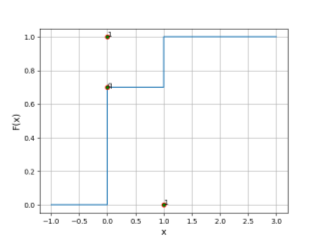
\includegraphics[scale=1]{figures/Figure_1.png} 
	     \caption{if p=0.3}
	     \label{figure 1}
        \end{figure}	     
	\end{frame}
	
\end{document}